\section{Diagramme des exercices}

Nous pr�sentons ici la gestion des exercices.\\

Pour commencer, voyons un aper�u des diff�rentes classes entrants en
jeu :
\begin{center}
\scalebox{0.6}{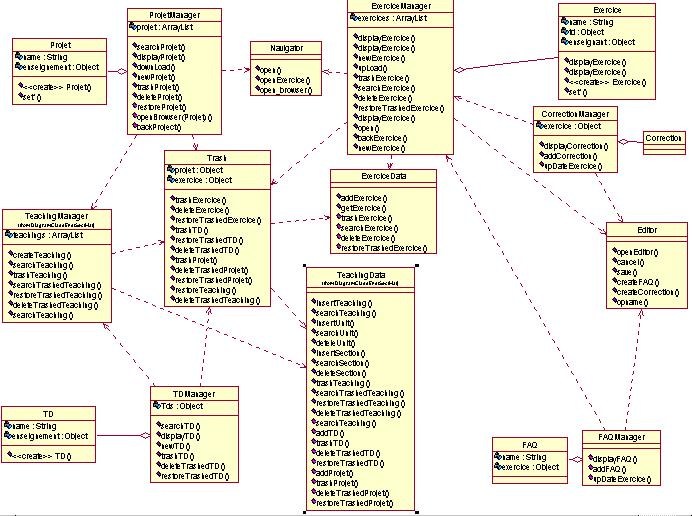
\includegraphics{images/ex_td_proj_Class.jpg}}\\
\par Diagramme de classes.\\
\end{center}

\begin{itemize}
\item Exercice : Repr�sente un objet contenant les donn�es d'un
exercice. Apr�s sa cr�ation, il est stock� dans ExerciceManager.\\

\item ExerciceManager : C'est l'objet qui g�re les exercices, il
s'occupe de leur cr�ation, recherche.\\

\item ExerciceData : Il g�re le stockage des exercices dans
leur int�gralit�. Le ExerciceManager lui fait appel pour toutes les
op�rations.\\

\item Trash : C'est l'objet qui collecte tous les
exercices mis � la poubelle par leur cr�ateurs. Il les conserve
jusqu'a leur suppression d�finitive.\\

\item FAQManager : Il g�re l'ensemble des Foire Aux Questions et int�ragit
avec le ExerciceManager pour la cr�ation ou la suppression de FAQ dans
un exercice donn�.\\

\item CorrectionManager : Il g�re l'ensemble des corrections et int�ragit
avec le ExerciceManager pour la cr�ation ou la suppression de correction dans
un exercice donn�.
\end{itemize}
\begin{center}
\scalebox{0.6}{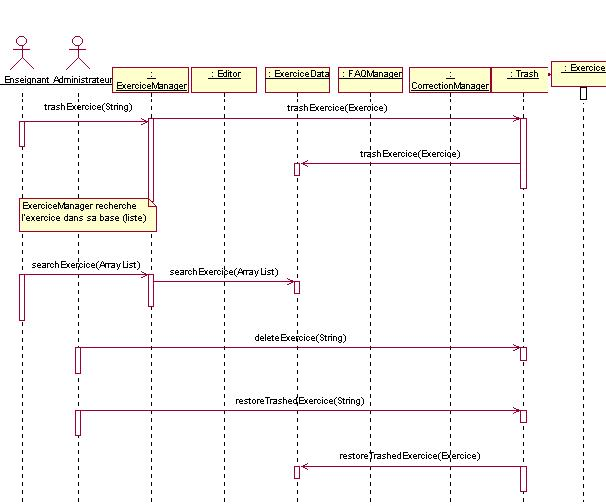
\includegraphics{images/exo_trash_search.jpg}}\\
\par Diagramme de s�quence de la recherche et de la suppression des exercices\newpage 
\scalebox{0.6}{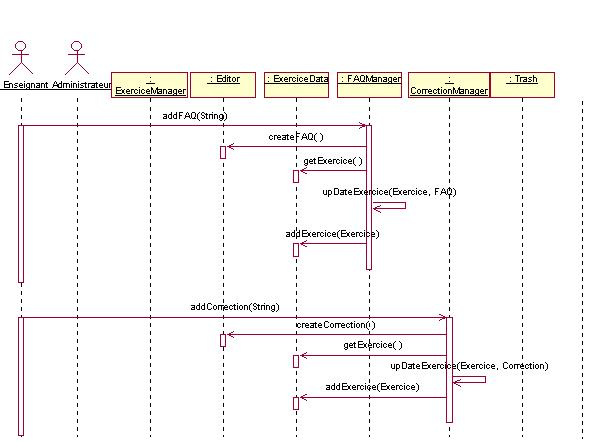
\includegraphics{images/exo_faq_correction.jpg}}\\
\par Diagramme de s�quence de la FAQ et de la correction\\
\scalebox{0.6}{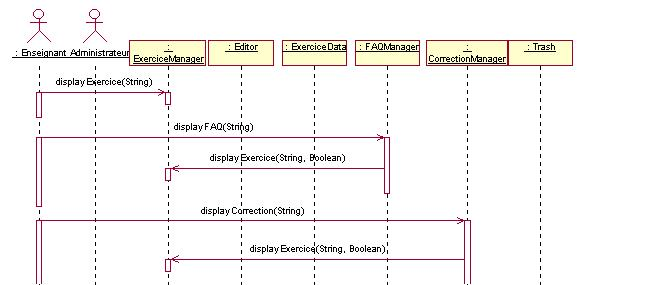
\includegraphics{images/exo_display.jpg}}\\
\par Diagramme de s�quence de l'affichage\newpage
\scalebox{0.6}{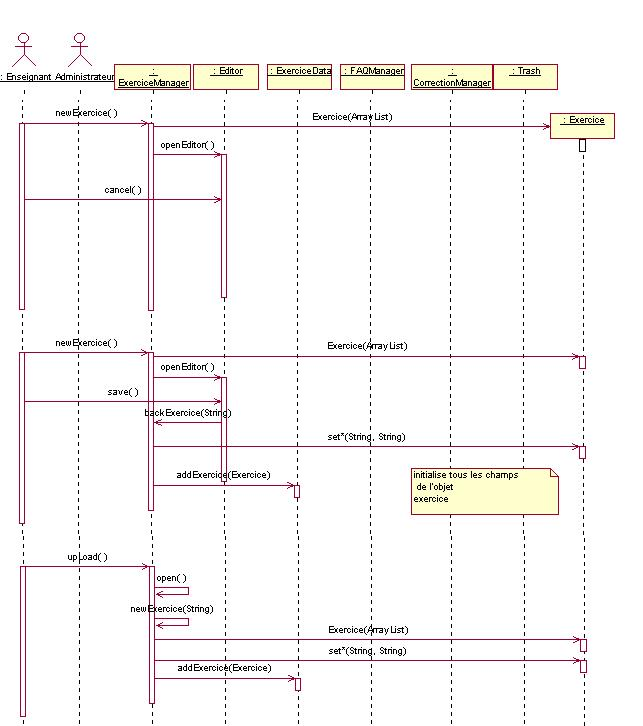
\includegraphics{images/exo_new.jpg}}\\
\par Diagramme de s�quence de la cr�ation.\\
\end{center}
